\subsection{Setup}\label{sec:setup}
\paragraph{Datasets.} We use four image datasets of increasing difficulty: MNIST~\citep{lecun1998mnist}, Fashion-MNIST~\citep{xiao2017fmnist} (the main benchmark), SVHN~\citep{netzer2011svhn} (natural photographs of house numbers) and CIFAR-10~\citep{krizhevsky2009cifar} (natural object images). Federations are built from them following the non-IID taxonomy used in the survey~\citep{benali2026survey}, which lists image classification with rotations and label swaps as the standard CFL benchmark~\citep[Table~6]{benali2026survey}.

\paragraph{Heterogeneity.} Each client belongs to a latent concept group. \emph{Concept shift on features} is a rotation of the inputs (by $0^\circ,90^\circ,180^\circ,270^\circ$, or by $0,\theta,2\theta,3\theta$ in the strength sweep). \emph{Concept shift on targets} is a label permutation that swaps two pairs of classes per group. On top of this, every client has \emph{target skew} (Dirichlet label proportions, $\alpha=0.3$, or $\alpha=0.1$ in the label-only scenario) and, where indicated, \emph{quantity skew} (log-normal dataset sizes with $\sigma=1$, clipped to $[30,3200]$, mean 400). Table~\ref{tab:scenarios} lists all scenarios. Each client has a local test set drawn with its own label proportions and transformation. We also evaluate every model on a class-balanced test set of its client's concept (\emph{concept accuracy}), which measures generalisation beyond the local label mix.

\begin{table}[!htbp]
\centering
\caption{Scenarios. $N$: clients; groups: number of concept groups; QS: quantity skew; part.: fraction of clients per round.}\label{tab:scenarios}
\small
\resizebox{\textwidth}{!}{%
\begin{tabular}{llllcl}
\toprule
Scenario & Dataset(s) & Concept groups & $N$ & QS & Other \\
\midrule
Rotation & FMNIST, MNIST, SVHN, CIFAR-10 & 4 rotations ($90^\circ$ steps) & 40 & -- & \\
Label swap & FMNIST, MNIST, SVHN, CIFAR-10 & 4 labelings (2 swapped pairs) & 40 & -- & \\
Rotation + QS & FMNIST & 4 rotations & 40 & \checkmark & \\
Mixed + QS & FMNIST & 2 rotations $\times$ 2 labelings & 40 & \checkmark & \\
Label skew only & FMNIST & 1 (true $K=1$) & 40 & \checkmark & $\alpha=0.1$ \\
Minority groups & FMNIST & 4 rotations, 25/9/4/2 clients & 40 & -- & \\
Strength $\theta$ & FMNIST & 4 rotations, $\theta\in\{15^\circ,30^\circ,45^\circ\}$ & 40 & -- & \\
Groups $K$ & FMNIST & $K\in\{2,4,8\}$ labelings & 40 & -- & \\
Partial participation & FMNIST & rotation / label swap & 40 & -- & part.\ $=0.3$ \\
Scale & FMNIST & 4 rotations & 200 & -- & 200 samples/client \\
\bottomrule
\end{tabular}}
\end{table}

\paragraph{Training.} All methods use the same CNN (two convolutional and two fully connected layers; $d=46{,}730$ parameters for $28\times28$ inputs and $65{,}962$ for $32\times32$ colour images), SGD with learning rate $0.05$, batch size 32, one local epoch per round and 50 communication rounds. Methods with a warm-up (DisCo-CFL, FL+HC, FeSEM, Oracle) spend 10 of the 50 rounds on FedAvg. \emph{Local} trains each client alone for 50 epochs. Every configuration is run with three seeds, which change the federation, the initialisation and the sketch: 618 training runs in total, plus the clustering-only studies.

\paragraph{Baselines.} We compare with nine methods that cover all three families of the taxonomy and the main alternatives to clustering:
\begin{itemize}[leftmargin=*,itemsep=1pt]
\item \emph{Single model / personalisation:} FedAvg~\citep{mcmahan2017fedavg}; Local; FedAvg-FT (FedAvg followed by one epoch of local fine-tuning, a standard personalisation baseline).
\item \emph{Client-side:} IFCA~\citep{ghosh2020ifca}.
\item \emph{Server-side:} CFL/MTCFL~\citep{sattler2021cfl} (recursive cosine bipartitioning, triggered when the norm of the aggregated update falls below $\varepsilon_1=0.9$ times the mean client-update norm); FL+HC~\citep{briggs2020flhc} (Ward clustering of local updates after the warm-up); FeSEM~\citep{long2023fesem} (EM-like assignment to the nearest of $K$ centres in parameter space, with the same warm-up and a $k$-means++ initialisation on the clients' local models).
\item \emph{Metadata-based:} PACFL~\citep{vahidian2023pacfl} (principal angles between client data subspaces, $p=3$).
\item \emph{Oracle:} FedAvg inside the ground-truth groups (an upper reference).
\end{itemize}
IFCA, FL+HC, FeSEM and PACFL are \emph{given the true number of groups} $K$, which favours them. DisCo-CFL and MTCFL find $K$ on their own. The MTCFL thresholds and the FeSEM initialisation were selected on the same pilot run as DisCo-CFL. Without them, MTCFL never splits and FeSEM collapses to a single cluster.

\paragraph{DisCo-CFL.} Sketch dimension $p=1024$, at most 200 samples per class for the signature, classes with fewer than 4 samples not reported, $\tau=0.8$, $\lambda=0.5$, $e_{\min}=0.05$, low-evidence threshold $0.3$, $z=2$, per-sample clipping $C_{\rm clip}=0.5$. These values, and the design choices of bottleneck linkage and evidence-ordered merging, were fixed during pilot runs on seed 0 of the Rotation, Label swap, Mixed + QS and label-only configurations (and seed 1 of Label swap with QS), using clustering quality only. They are kept identical for all scenarios, seeds and datasets. Seeds 1 and 2, the sweeps, and the MNIST, SVHN and CIFAR-10 results were not used for design. Per-sample clipping ($C_{\rm clip}$ chosen on seed 0 only, from $\{0.5,1,2\}$ in all scenarios and additionally $\{0.1,0.25\}$ in the label-only scenario) was added after a first sensitivity study showed over-splitting caused by heavy-tailed per-sample gradients. The run without clipping is reported as an ablation. On the colour datasets we also report DisCo-T30, which uses 30 warm-up rounds (Section~\ref{sec:datasets}). The sensitivity to $\tau$ is reported in the main paper and the sensitivity to $\lambda$ in Table~\ref{tab:lambda}.

\paragraph{Metrics.} \emph{Performance:} mean local test accuracy (Acc), with the prior correction of Section~\ref{sec:pc} applied identically to every method, and concept accuracy. \emph{Fairness:} accuracy of the worst 10\% of clients (Acc@10\%), accuracy of the worst concept group (Worst-grp), Jain's index. \emph{Clustering:} ARI with respect to the groups, number of clusters $K$, and the \emph{conflict-merge rate}: the fraction of conflicting client pairs (Definition~\ref{def:concept}) that end up in the same cluster. ARI penalises the legitimate placement of compatible clients (e.g.\ a client of a label-swap group that holds none of the swapped classes), whereas the conflict-merge rate measures exactly the harmful errors. \emph{Statistics:} paired one-sided Wilcoxon signed-rank tests of DisCo-CFL against each baseline over all (scenario, seed) pairs.

\subsection{Full results on Fashion-MNIST}\label{sec:fullfmnist}
Table~\ref{tab:main} reports all metrics on Fashion-MNIST for the ten methods. Accuracy is \emph{with} the prior correction~\eqref{eq:pc}, applied identically to every method; the uncorrected mean accuracy is shown in the first column.

\begin{table}[!htbp]
\centering
\caption{Fashion-MNIST, 40 clients, 3 seeds. Acc: mean local accuracy (with prior correction, $\pm$ std over seeds). Acc (raw): without correction. Acc@10\%: mean accuracy of the worst 10\% of clients. Worst-grp: accuracy of the worst concept group. Concept: accuracy on the class-balanced test set of the client's concept. Conflict\%: fraction of conflicting client pairs merged into one cluster (lower is better). IFCA, FeSEM, FL+HC and PACFL receive the true $K$; DisCo-CFL finds it. Oracle uses the ground-truth groups. Best non-oracle values in bold.}\label{tab:main}
\scriptsize
\setlength{\tabcolsep}{3.2pt}
\begin{tabular}{lccccccccc}
\toprule
Method & Acc (raw) & Acc & Acc@10\% & Worst-grp & Concept & Jain & ARI & K & Conflict\% \\
\midrule
\multicolumn{10}{l}{\textit{Rotation}}\\
FedAvg & 76.6 & 86.0$\pm$0.5 & 76.5 & 82.9 & 75.7 & 0.99 & 0.00 & 1.0 & 100.0 \\
Local & 87.8 & 87.8$\pm$0.7 & 80.8 & 86.9 & 60.7 & \textbf{1.00} & 0.00 & 40.0 & \textbf{0.0} \\
FedAvg-FT & 88.8 & 88.8$\pm$0.5 & 81.5 & 88.0 & 77.9 & \textbf{1.00} & 0.00 & 40.0 & \textbf{0.0} \\
IFCA & 83.5 & 89.2$\pm$1.0 & 80.9 & 86.7 & 77.0 & \textbf{1.00} & 0.41 & 4.0 & 22.0 \\
FeSEM & 83.0 & 89.1$\pm$0.3 & 80.8 & 87.8 & 80.6 & \textbf{1.00} & 0.67 & 4.0 & 10.4 \\
MTCFL & 89.4 & 90.2$\pm$0.6 & 83.6 & 89.1 & 73.9 & \textbf{1.00} & 0.15 & 34.7 & \textbf{0.0} \\
FL+HC & 78.5 & 86.4$\pm$0.4 & 76.9 & 83.6 & 74.9 & 0.99 & 0.01 & 4.0 & 85.0 \\
PACFL & 82.8 & 89.5$\pm$0.8 & 81.8 & 87.8 & 79.4 & \textbf{1.00} & 0.48 & 4.0 & 21.0 \\
DisCo & 84.5 & \textbf{90.5$\pm$0.4} & \textbf{84.6} & \textbf{89.5} & \textbf{83.9} & \textbf{1.00} & \textbf{1.00} & 4.0 & \textbf{0.0} \\
Oracle & 84.5 & 90.5$\pm$0.4 & 84.6 & 89.5 & 83.9 & 1.00 & 1.00 & 4.0 & 0.0 \\
\midrule
\multicolumn{10}{l}{\textit{Label swap}}\\
FedAvg & 54.2 & 70.1$\pm$1.4 & 47.2 & 58.6 & 55.7 & 0.94 & 0.00 & 1.0 & 100.0 \\
Local & 88.7 & 88.7$\pm$0.7 & 80.1 & 87.0 & 64.0 & \textbf{1.00} & 0.00 & 40.0 & \textbf{0.0} \\
FedAvg-FT & 90.6 & 90.6$\pm$0.5 & 84.1 & \textbf{89.7} & 80.9 & \textbf{1.00} & 0.00 & 40.0 & \textbf{0.0} \\
IFCA & 76.9 & 85.6$\pm$1.6 & 72.6 & 79.4 & 71.1 & 0.99 & 0.45 & 4.0 & 17.1 \\
FeSEM & 80.4 & 87.5$\pm$5.0 & 76.3 & 83.0 & 79.8 & 0.99 & 0.87 & 4.0 & 5.7 \\
MTCFL & 88.2 & 90.4$\pm$0.6 & 84.3 & 87.8 & 76.1 & 0.99 & 0.30 & 29.0 & 2.8 \\
FL+HC & 58.4 & 71.5$\pm$1.1 & 47.0 & 61.1 & 59.1 & 0.93 & 0.01 & 4.0 & 85.7 \\
PACFL & 57.9 & 74.8$\pm$2.6 & 50.7 & 67.8 & 53.6 & 0.94 & -0.01 & 4.0 & 34.9 \\
DisCo & 85.4 & \textbf{90.8$\pm$0.3} & \textbf{84.6} & 89.2 & \textbf{84.9} & \textbf{1.00} & \textbf{1.00} & 4.0 & \textbf{0.0} \\
Oracle & 85.4 & 90.8$\pm$0.3 & 84.6 & 89.2 & 84.9 & 1.00 & 1.00 & 4.0 & 0.0 \\
\midrule
\multicolumn{10}{l}{\textit{Rotation + QS}}\\
FedAvg & 75.9 & 85.8$\pm$0.3 & 78.4 & 82.6 & 74.7 & \textbf{1.00} & 0.00 & 1.0 & 100.0 \\
Local & 87.9 & 87.9$\pm$1.2 & 80.4 & 84.9 & 61.9 & \textbf{1.00} & 0.00 & 40.0 & \textbf{0.0} \\
FedAvg-FT & 87.6 & 87.6$\pm$0.7 & 80.8 & 84.8 & 75.4 & 0.99 & 0.00 & 40.0 & \textbf{0.0} \\
IFCA & 82.3 & 88.5$\pm$0.6 & 81.7 & 86.1 & 77.0 & \textbf{1.00} & 0.44 & 3.3 & 24.3 \\
FeSEM & 81.2 & 88.3$\pm$0.6 & 81.6 & 85.5 & 78.4 & 0.99 & 0.66 & 4.0 & 11.6 \\
MTCFL & 85.4 & 88.8$\pm$0.7 & 82.7 & 86.7 & 73.5 & \textbf{1.00} & 0.32 & 20.7 & 15.6 \\
FL+HC & 76.9 & 85.3$\pm$1.0 & 76.1 & 80.2 & 73.5 & 0.99 & 0.01 & 4.0 & 85.0 \\
PACFL & 80.1 & 88.0$\pm$1.8 & 79.7 & 84.3 & 76.5 & 0.99 & 0.44 & 4.0 & 20.8 \\
DisCo & 83.3 & \textbf{90.1$\pm$0.2} & \textbf{84.5} & \textbf{88.7} & \textbf{82.1} & \textbf{1.00} & \textbf{1.00} & 4.0 & \textbf{0.0} \\
Oracle & 83.3 & 90.1$\pm$0.2 & 84.5 & 88.7 & 82.1 & 1.00 & 1.00 & 4.0 & 0.0 \\
\bottomrule
\end{tabular}

\end{table}

\begin{table}[!htbp]
\centering
\caption*{Table~\ref{tab:main} (continued).}
\scriptsize
\setlength{\tabcolsep}{3.2pt}
\begin{tabular}{lccccccccc}
\toprule
Method & Acc (raw) & Acc & Acc@10\% & Worst-grp & Concept & Jain & ARI & K & Conflict\% \\
\midrule
\multicolumn{10}{l}{\textit{Mixed + QS}}\\
FedAvg & 70.2 & 80.8$\pm$0.9 & 66.3 & 75.1 & 66.6 & 0.98 & 0.00 & 1.0 & 100.0 \\
Local & 88.9 & 88.9$\pm$1.3 & 82.7 & 86.6 & 64.1 & \textbf{1.00} & 0.00 & 40.0 & \textbf{0.0} \\
FedAvg-FT & 88.6 & 88.6$\pm$0.9 & 82.9 & 85.7 & 76.5 & 0.99 & 0.00 & 40.0 & \textbf{0.0} \\
IFCA & 82.5 & 89.0$\pm$0.3 & 82.5 & 87.5 & 75.4 & \textbf{1.00} & 0.34 & 3.7 & 25.5 \\
FeSEM & 81.1 & 88.1$\pm$1.3 & 79.4 & 85.4 & 77.9 & 0.99 & 0.67 & 4.0 & 8.3 \\
MTCFL & 78.4 & 84.8$\pm$1.8 & 70.0 & 76.8 & 70.2 & 0.98 & 0.24 & 16.3 & 29.3 \\
FL+HC & 72.0 & 81.8$\pm$0.3 & 68.6 & 77.4 & 67.1 & 0.98 & 0.01 & 4.0 & 85.4 \\
PACFL & 71.5 & 83.3$\pm$0.4 & 68.3 & 79.3 & 66.4 & 0.98 & 0.20 & 4.0 & 21.8 \\
DisCo & 84.5 & \textbf{90.6$\pm$0.3} & \textbf{84.3} & \textbf{88.8} & \textbf{82.5} & \textbf{1.00} & \textbf{0.94} & 4.0 & 0.6 \\
Oracle & 84.2 & 90.6$\pm$0.3 & 84.6 & 88.7 & 83.4 & 1.00 & 1.00 & 4.0 & 0.0 \\
\midrule
\multicolumn{10}{l}{\textit{Label skew only}}\\
FedAvg & 87.6 & 95.5$\pm$0.4 & \textbf{90.9} & 95.5 & 85.8 & \textbf{1.00} & \textbf{1.00} & 1.0 & \textbf{0.0} \\
Local & 94.6 & 94.6$\pm$0.2 & 87.7 & 94.6 & 51.0 & \textbf{1.00} & 0.00 & 40.0 & \textbf{0.0} \\
FedAvg-FT & 94.2 & 94.2$\pm$0.3 & 90.1 & 94.2 & 80.7 & \textbf{1.00} & 0.00 & 40.0 & \textbf{0.0} \\
IFCA & 87.7 & 95.4$\pm$0.6 & 90.7 & 95.4 & 85.7 & \textbf{1.00} & \textbf{1.00} & 1.0 & \textbf{0.0} \\
FeSEM & 87.7 & 95.5$\pm$0.4 & 90.6 & 95.5 & 85.7 & \textbf{1.00} & \textbf{1.00} & 1.0 & \textbf{0.0} \\
MTCFL & 92.0 & 95.3$\pm$0.2 & 88.5 & 95.3 & 77.1 & \textbf{1.00} & 0.00 & 20.7 & \textbf{0.0} \\
FL+HC & 87.5 & 95.5$\pm$0.5 & 90.4 & 95.5 & \textbf{85.9} & \textbf{1.00} & \textbf{1.00} & 1.0 & \textbf{0.0} \\
PACFL & 87.6 & 95.5$\pm$0.4 & \textbf{90.9} & 95.5 & 85.8 & \textbf{1.00} & \textbf{1.00} & 1.0 & \textbf{0.0} \\
DisCo & 87.6 & \textbf{95.6$\pm$0.4} & 90.8 & \textbf{95.6} & 85.6 & \textbf{1.00} & 0.67 & 1.3 & \textbf{0.0} \\
Oracle & 87.6 & 95.5$\pm$0.4 & 90.9 & 95.5 & 85.8 & 1.00 & 1.00 & 1.0 & 0.0 \\
\midrule
\multicolumn{10}{l}{\textit{Minority groups}}\\
FedAvg & 77.0 & 85.5$\pm$0.7 & 74.1 & 35.7 & 76.7 & 0.98 & 0.00 & 1.0 & 100.0 \\
Local & 88.5 & 88.5$\pm$0.5 & 81.0 & 85.2 & 62.7 & \textbf{1.00} & 0.00 & 40.0 & \textbf{0.0} \\
FedAvg-FT & 89.4 & 89.4$\pm$0.5 & 82.9 & 81.7 & 78.5 & \textbf{1.00} & 0.00 & 40.0 & \textbf{0.0} \\
IFCA & 83.6 & 89.4$\pm$1.7 & 81.2 & 67.3 & 78.1 & 0.99 & 0.57 & 3.7 & 22.8 \\
FeSEM & 84.0 & 89.8$\pm$0.7 & 82.0 & 79.4 & 81.8 & \textbf{1.00} & 0.62 & 4.0 & 5.7 \\
MTCFL & 82.0 & 87.3$\pm$3.1 & 78.0 & 51.9 & 76.7 & 0.98 & 0.04 & 11.3 & 66.7 \\
FL+HC & 80.4 & 87.7$\pm$0.8 & 78.0 & 74.5 & 78.0 & 0.99 & 0.22 & 4.0 & 74.8 \\
PACFL & 83.1 & 89.8$\pm$0.7 & 83.9 & 82.7 & 78.8 & \textbf{1.00} & 0.43 & 4.0 & 17.8 \\
DisCo & 85.3 & \textbf{90.8$\pm$0.6} & \textbf{85.3} & \textbf{86.5} & \textbf{84.1} & \textbf{1.00} & \textbf{0.98} & 4.3 & \textbf{0.0} \\
Oracle & 85.3 & 90.9$\pm$0.6 & 85.3 & 86.5 & 84.2 & 1.00 & 1.00 & 4.0 & 0.0 \\
\bottomrule
\end{tabular}

\end{table}

\paragraph{DisCo-CFL recovers the concept structure without being told $K$.} In \emph{Rotation}, \emph{Label swap} and \emph{Rotation + QS}, DisCo-CFL finds exactly the ground-truth partition in all seeds (ARI $=1$) and matches the Oracle on every metric. In \emph{Mixed + QS}, where two groups differ only on 4 of the 10 classes, it reaches ARI $0.94$ with $0.6\%$ conflicting pairs merged. In \emph{Minority groups} (25/9/4/2 clients) it reaches ARI $0.98$ with no conflicts. The baselines that are given the true $K$ merge 6--86\% of the conflicting pairs: FeSEM 6--12\%, IFCA 17--26\%, PACFL 18--35\% and FL+HC 75--86\%. CFL/MTCFL has few conflicts only in the scenarios where it fragments the federation into 16--35 clusters. FL+HC groups clients by label proportions instead of concepts, PACFL by the pixel subspace (which a label swap leaves unchanged), IFCA suffers from initialisation, and FeSEM, the strongest clustering baseline, confuses nearby groups in parameter space.

\paragraph{Fairness.} DisCo-CFL has the best accuracy on the worst 10\% of clients in every scenario with concept shift, and the best worst-group accuracy in all of them except \emph{Label swap}, where FedAvg-FT is 0.5 points higher (89.7\% vs.\ 89.2\%). The gap is largest for minority concepts. In \emph{Minority groups}, the worst concept group reaches 86.5\% with DisCo-CFL, against 35.7\% with FedAvg, 51.9\% with MTCFL, 67.3\% with IFCA, 74.5\% with FL+HC and 79.4\% with FeSEM: the size-independence of Corollary~\ref{cor:sc} in practice. Table~\ref{tab:minority} isolates the clustering step. DisCo-CFL recovers minority groups of 1, 2, 3 and 5 clients with recall and purity $1.00$ and no conflicting merges. FL+HC isolates the minority only by spending its fixed $K$ on it while merging 81\% of the conflicting pairs among the majority groups, and PACFL does not find the minority at all.

\begin{table}[!htbp]
\centering
\caption{Minority-group recovery (clustering step only; groups of 20/10/10/$m$ clients; 3 seeds).}\label{tab:minority}
\small
\begin{tabular}{lcccccc}
\toprule
& \multicolumn{3}{c}{DisCo-CFL} & \multicolumn{3}{c}{FL+HC ($K$ given)} \\
\cmidrule(lr){2-4}\cmidrule(lr){5-7}
$m$ & recall & ARI & conflict\% & recall & ARI & conflict\% \\
\midrule
1 & 1.00 & 0.98 & 0.0 & 1.00 & 0.09 & 81.5\\
2 & 1.00 & 0.98 & 0.0 & 1.00 & 0.11 & 81.0\\
3 & 1.00 & 1.00 & 0.0 & 1.00 & 0.12 & 80.6\\
5 & 1.00 & 0.98 & 0.0 & 0.60 & 0.09 & 82.9\\
\bottomrule
\end{tabular}
\end{table}

\subsection{Other datasets: MNIST, SVHN and CIFAR-10}\label{sec:datasets}
Table~\ref{tab:other} repeats the two basic concept-shift scenarios on MNIST, SVHN and CIFAR-10 with the same hyperparameters.

\paragraph{MNIST and SVHN.} On both datasets DisCo-CFL recovers the groups (ARI $0.97$--$1.00$), never merges conflicting clients, and reaches the accuracy of the Oracle within $0.1$ points. On SVHN, a harder dataset of natural photographs, its concept accuracy is 79.7\% (rotation) and 82.5\% (label swap), against at most 75.6\% and 72.7\% for any baseline. FeSEM is the strongest clustering baseline on these datasets (ARI $0.66$--$0.98$), and FedAvg-FT the strongest non-clustering one. Both remain 0.7--11.6 points below DisCo-CFL in concept accuracy. In the MNIST rotation scenario, two seeds leave one or two clients in singleton clusters. These clients are flagged as anomalous (mean ARI $0.97$, $K=5.0$) and train alone; the mean accuracy still equals the Oracle's.

\paragraph{CIFAR-10.} CIFAR-10 is harder, and here DisCo-CFL is not the best method on every metric. With the default 10 warm-up rounds the reference model is only about 40\% accurate. Its class-conditional gradients then depend little on the orientation of most natural-image classes: the mean between-group similarity is 0.83--0.90, and only vehicle classes separate clearly. The separation $\Delta$ of Assumption~\ref{ass:sep} is therefore small. For label swaps DisCo-CFL still reaches ARI $0.87$ and a higher concept accuracy than every baseline (48.6\%), but for rotations it reaches only ARI $0.38$. The theory points to the remedy, a more informative reference model. With 30 warm-up rounds (DisCo-T30), ARI rises to $0.74$ (rotation) and $0.92$ (label swap), conflicting merges fall to 4.2\% and 0.1\%, and concept accuracy is 44.8\% and 49.8\%. That is the best of all non-oracle methods in both scenarios, tied with FeSEM on rotation. Table~\ref{tab:warm} gives the clustering-only trend. CFL/MTCFL has the highest \emph{local} accuracy on CIFAR-10 (67.0\% and 68.8\%, above the Oracle's 64.2\% and 64.7\%). It splits the federation into 33--35 clusters and personalises to each client's label mix with the small CNN, and its concept accuracy is 7--8 points below DisCo-T30's.

\begin{table}[!htbp]
\centering
\caption{CIFAR-10 rotation, clustering step only: effect of the warm-up length $T_0$ (3 seeds).}\label{tab:warm}
\small
\begin{tabular}{lccc}
\toprule
$T_0$ & ARI & $K$ & conflict\% \\
\midrule
10 & 0.37 & 3.7 & 24.8 \\
20 & 0.64 & 5.0 & 8.9 \\
30 & 0.74 & 4.7 & 4.2 \\
\bottomrule
\end{tabular}
\end{table}

\begin{table}[!htbp]
\centering
\caption{MNIST, SVHN and CIFAR-10 (40 clients, 3 seeds; same settings and columns as Table~\ref{tab:main}). DisCo-T30: DisCo-CFL with 30 warm-up rounds.}\label{tab:other}
\scriptsize
\setlength{\tabcolsep}{3.2pt}
\begin{tabular}{lccccccccc}
\toprule
Method & Acc (raw) & Acc & Acc@10\% & Worst-grp & Concept & Jain & ARI & K & Conflict\% \\
\midrule
\multicolumn{10}{l}{\textit{MNIST rotation}}\\
FedAvg & 91.8 & 94.7$\pm$0.6 & 91.1 & 92.4 & 90.6 & \textbf{1.00} & 0.00 & 1.0 & 100.0 \\
Local & 96.5 & 96.5$\pm$0.4 & 94.3 & 96.1 & 82.0 & \textbf{1.00} & 0.00 & 40.0 & \textbf{0.0} \\
FedAvg-FT & 97.2 & 97.2$\pm$0.1 & 95.5 & 97.0 & 94.6 & \textbf{1.00} & 0.00 & 40.0 & \textbf{0.0} \\
IFCA & 95.5 & 96.9$\pm$0.5 & 94.4 & 95.6 & 91.2 & \textbf{1.00} & 0.42 & 4.0 & 21.6 \\
FeSEM & 97.3 & 98.2$\pm$0.1 & 97.0 & 97.8 & 95.9 & \textbf{1.00} & 0.78 & 4.0 & 5.3 \\
MTCFL & 93.8 & 95.7$\pm$0.7 & 92.8 & 92.9 & 90.8 & \textbf{1.00} & 0.09 & 9.7 & 58.9 \\
FL+HC & 91.4 & 94.3$\pm$0.9 & 88.4 & 91.6 & 89.9 & \textbf{1.00} & 0.01 & 4.0 & 85.0 \\
PACFL & 95.1 & 96.8$\pm$0.3 & 94.5 & 95.7 & 91.6 & \textbf{1.00} & 0.45 & 4.0 & 15.9 \\
DisCo & 97.6 & \textbf{98.5$\pm$0.1} & \textbf{97.3} & \textbf{98.3} & \textbf{97.1} & \textbf{1.00} & \textbf{0.97} & 5.0 & \textbf{0.0} \\
Oracle & 97.6 & 98.5$\pm$0.1 & 97.3 & 98.3 & 97.2 & 1.00 & 1.00 & 4.0 & 0.0 \\
\midrule
\multicolumn{10}{l}{\textit{MNIST label swap}}\\
FedAvg & 60.4 & 78.5$\pm$2.3 & 52.8 & 61.9 & 60.9 & 0.94 & 0.00 & 1.0 & 100.0 \\
Local & 97.1 & 97.1$\pm$0.2 & 95.0 & 96.4 & 86.0 & \textbf{1.00} & 0.00 & 40.0 & \textbf{0.0} \\
FedAvg-FT & 98.1 & 98.1$\pm$0.0 & 96.8 & 97.5 & 92.0 & \textbf{1.00} & 0.00 & 40.0 & \textbf{0.0} \\
IFCA & 90.9 & 95.8$\pm$0.6 & 92.4 & 90.4 & 87.9 & \textbf{1.00} & 0.60 & 3.7 & 13.3 \\
FeSEM & 97.4 & 98.4$\pm$0.4 & 97.6 & 97.4 & 97.1 & \textbf{1.00} & 0.98 & 4.0 & 0.6 \\
MTCFL & 85.7 & 91.7$\pm$3.2 & 82.2 & 85.0 & 78.7 & 0.98 & 0.24 & 18.0 & 24.2 \\
FL+HC & 66.0 & 80.8$\pm$2.0 & 56.6 & 69.6 & 65.9 & 0.95 & 0.01 & 4.0 & 85.7 \\
PACFL & 67.2 & 83.3$\pm$2.1 & 62.2 & 75.5 & 63.4 & 0.97 & 0.00 & 4.0 & 30.0 \\
DisCo & 97.9 & \textbf{98.7$\pm$0.1} & \textbf{97.7} & \textbf{98.5} & \textbf{97.8} & \textbf{1.00} & \textbf{1.00} & 4.0 & \textbf{0.0} \\
Oracle & 97.9 & 98.7$\pm$0.1 & 97.7 & 98.5 & 97.8 & 1.00 & 1.00 & 4.0 & 0.0 \\
\midrule
\multicolumn{10}{l}{\textit{SVHN rotation}}\\
FedAvg & 63.3 & 72.4$\pm$1.2 & 58.1 & 64.5 & 63.4 & 0.98 & 0.00 & 1.0 & 100.0 \\
Local & 77.5 & 77.5$\pm$1.0 & 69.0 & 75.6 & 43.9 & 0.99 & 0.00 & 40.0 & \textbf{0.0} \\
FedAvg-FT & 81.9 & 81.9$\pm$0.2 & 77.1 & 81.0 & 69.5 & \textbf{1.00} & 0.00 & 40.0 & \textbf{0.0} \\
IFCA & 74.8 & 80.2$\pm$1.6 & 71.5 & 76.9 & 65.9 & 0.99 & 0.26 & 3.7 & 25.8 \\
FeSEM & 79.8 & 84.1$\pm$0.3 & 79.0 & 82.3 & 75.6 & \textbf{1.00} & 0.66 & 4.0 & 9.4 \\
MTCFL & 82.4 & 84.0$\pm$0.2 & 79.9 & 83.0 & 66.9 & \textbf{1.00} & 0.27 & 24.7 & 10.6 \\
FL+HC & 65.3 & 72.9$\pm$1.4 & 57.6 & 64.9 & 64.4 & 0.98 & 0.01 & 4.0 & 85.0 \\
PACFL & 70.2 & 78.1$\pm$1.3 & 67.7 & 75.9 & 67.5 & 0.99 & 0.39 & 4.0 & 16.9 \\
DisCo & 81.3 & \textbf{85.4$\pm$0.2} & \textbf{80.4} & \textbf{83.9} & \textbf{79.7} & \textbf{1.00} & \textbf{0.99} & 4.3 & \textbf{0.0} \\
DisCo-T30 & 80.7 & 84.6$\pm$0.3 & \textbf{80.4} & 83.5 & 78.6 & \textbf{1.00} & 0.93 & 5.7 & \textbf{0.0} \\
Oracle & 81.5 & 85.5$\pm$0.3 & 80.5 & 84.3 & 80.0 & 1.00 & 1.00 & 4.0 & 0.0 \\
\bottomrule
\end{tabular}

\end{table}

\begin{table}[!htbp]
\centering
\caption*{Table~\ref{tab:other} (continued).}
\scriptsize
\setlength{\tabcolsep}{3.2pt}
\begin{tabular}{lccccccccc}
\toprule
Method & Acc (raw) & Acc & Acc@10\% & Worst-grp & Concept & Jain & ARI & K & Conflict\% \\
\midrule
\multicolumn{10}{l}{\textit{SVHN label swap}}\\
FedAvg & 52.6 & 64.5$\pm$3.7 & 44.9 & 54.5 & 50.9 & 0.94 & 0.00 & 1.0 & 100.0 \\
Local & 81.0 & 81.0$\pm$1.0 & 75.0 & 79.7 & 50.4 & \textbf{1.00} & 0.00 & 40.0 & \textbf{0.0} \\
FedAvg-FT & 84.9 & 84.9$\pm$0.1 & 79.8 & 84.3 & 72.7 & \textbf{1.00} & 0.00 & 40.0 & \textbf{0.0} \\
IFCA & 71.4 & 79.0$\pm$2.6 & 65.2 & 74.9 & 64.1 & 0.98 & 0.37 & 4.0 & 21.2 \\
FeSEM & 73.7 & 80.5$\pm$6.0 & 71.9 & 76.5 & 70.9 & 0.98 & 0.67 & 4.0 & 12.8 \\
MTCFL & 80.0 & 83.1$\pm$3.4 & 74.0 & 79.4 & 66.5 & 0.99 & 0.26 & 25.0 & 10.7 \\
FL+HC & 56.2 & 66.6$\pm$3.2 & 45.8 & 57.7 & 53.4 & 0.94 & 0.01 & 4.0 & 84.7 \\
PACFL & 54.2 & 69.1$\pm$1.9 & 53.6 & 60.3 & 48.2 & 0.97 & -0.01 & 4.0 & 28.9 \\
DisCo & 83.7 & \textbf{87.2$\pm$0.4} & \textbf{83.5} & 86.1 & \textbf{82.5} & \textbf{1.00} & \textbf{0.97} & 4.3 & \textbf{0.0} \\
DisCo-T30 & 83.8 & 87.1$\pm$0.2 & \textbf{83.5} & \textbf{86.4} & 82.1 & \textbf{1.00} & 0.94 & 5.7 & \textbf{0.0} \\
Oracle & 83.6 & 87.1$\pm$0.4 & 83.5 & 86.0 & 82.6 & 1.00 & 1.00 & 4.0 & 0.0 \\
\midrule
\multicolumn{10}{l}{\textit{CIFAR-10 rotation}}\\
FedAvg & 38.0 & 55.1$\pm$1.4 & 44.5 & 51.6 & 36.8 & 0.97 & 0.00 & 1.0 & 100.0 \\
Local & 56.2 & 56.2$\pm$3.6 & 42.7 & 52.1 & 21.0 & 0.96 & 0.00 & 40.0 & \textbf{0.0} \\
FedAvg-FT & 61.8 & 61.8$\pm$2.0 & 51.1 & 60.4 & 36.8 & \textbf{0.98} & 0.00 & 40.0 & \textbf{0.0} \\
IFCA & 45.9 & 56.5$\pm$1.6 & 44.1 & 53.4 & 32.0 & 0.97 & -0.01 & 4.0 & 32.2 \\
FeSEM & 49.4 & 61.9$\pm$1.5 & 52.3 & 59.0 & \textbf{44.8} & \textbf{0.98} & 0.69 & 4.0 & 12.1 \\
MTCFL & 65.6 & \textbf{67.0$\pm$2.2} & \textbf{56.8} & \textbf{63.3} & 38.2 & \textbf{0.98} & 0.14 & 34.7 & \textbf{0.0} \\
FL+HC & 40.5 & 55.6$\pm$1.6 & 43.5 & 54.4 & 36.9 & 0.97 & 0.01 & 4.0 & 85.0 \\
PACFL & 46.2 & 58.6$\pm$2.4 & 48.1 & 54.8 & 37.3 & \textbf{0.98} & 0.37 & 4.0 & 21.2 \\
DisCo & 47.6 & 60.5$\pm$1.2 & 47.5 & 56.3 & 41.0 & \textbf{0.98} & 0.38 & 3.7 & 24.6 \\
DisCo-T30 & 50.4 & 62.0$\pm$1.3 & 51.5 & 60.3 & \textbf{44.8} & \textbf{0.98} & \textbf{0.74} & 4.7 & 4.2 \\
Oracle & 52.0 & 64.2$\pm$1.7 & 54.3 & 61.6 & 47.4 & 0.99 & 1.00 & 4.0 & 0.0 \\
\midrule
\multicolumn{10}{l}{\textit{CIFAR-10 label swap}}\\
FedAvg & 34.8 & 51.0$\pm$2.9 & 36.0 & 43.0 & 33.5 & 0.95 & 0.00 & 1.0 & 100.0 \\
Local & 56.4 & 56.4$\pm$3.7 & 42.8 & 51.7 & 21.8 & 0.96 & 0.00 & 40.0 & \textbf{0.0} \\
FedAvg-FT & 64.5 & 64.5$\pm$2.7 & 53.9 & 62.9 & 40.8 & 0.98 & 0.00 & 40.0 & \textbf{0.0} \\
IFCA & 42.9 & 55.0$\pm$3.5 & 39.8 & 50.7 & 30.7 & 0.95 & 0.08 & 4.0 & 27.0 \\
FeSEM & 46.7 & 59.8$\pm$3.2 & 46.9 & 55.4 & 43.7 & 0.97 & 0.65 & 4.0 & 11.3 \\
MTCFL & 66.9 & \textbf{68.8$\pm$2.2} & \textbf{59.0} & \textbf{63.7} & 41.4 & 0.98 & 0.19 & 33.3 & 0.5 \\
FL+HC & 38.8 & 53.1$\pm$2.8 & 35.9 & 48.4 & 34.5 & 0.94 & 0.01 & 4.0 & 85.1 \\
PACFL & 35.3 & 52.0$\pm$2.7 & 37.2 & 46.1 & 29.9 & 0.95 & 0.00 & 4.0 & 45.4 \\
DisCo & 52.5 & 64.1$\pm$2.4 & 52.3 & 61.5 & 48.6 & 0.98 & 0.87 & 4.3 & 3.0 \\
DisCo-T30 & 54.7 & 64.6$\pm$2.2 & 54.9 & 62.4 & \textbf{49.8} & \textbf{0.99} & \textbf{0.92} & 5.0 & 0.1 \\
Oracle & 53.0 & 64.7$\pm$2.4 & 55.5 & 62.7 & 49.6 & 0.99 & 1.00 & 4.0 & 0.0 \\
\bottomrule
\end{tabular}

\end{table}

\subsection{Robustness sweeps}\label{sec:sweeps}
Table~\ref{tab:sweeps} varies one factor at a time on Fashion-MNIST: the strength of the concept shift, the number of groups, the fraction of participating clients and the number of clients. Baselines are given the true $K$ where they need it.

\begin{table}[!htbp]
\centering
\caption{Robustness sweeps (Fashion-MNIST, 3 seeds). For DisCo-CFL: ARI, number of clusters, conflict-merge rate, accuracy and concept accuracy. For comparison: the best baseline on accuracy and on concept accuracy (in parentheses), and the Oracle's accuracy.}\label{tab:sweeps}
\scriptsize
\setlength{\tabcolsep}{3pt}
\resizebox{\textwidth}{!}{%
\begin{tabular}{llcccccccc}
\toprule
& & \multicolumn{5}{c}{DisCo-CFL} & & & \\
\cmidrule(lr){3-7}
Factor & Setting & ARI & $K$ & Conflict\% & Acc & Concept & Best baseline Acc & Best baseline Concept & Oracle Acc \\
\midrule
Strength & $\theta=15^\circ$ & 0.42 & 3.0 & 32.1 & 90.0 & 82.8 & 90.2 (FeSEM) & 83.0 (FeSEM) & 90.5 \\
Strength & $\theta=30^\circ$ & 0.93 & 4.3 & 1.7 & 90.3 & 83.1 & 90.0 (PACFL) & 81.2 (PACFL) & 90.4 \\
Strength & $\theta=45^\circ$ & 1.00 & 4.0 & 0.0 & 90.4 & 83.8 & 89.9 (FeSEM) & 81.8 (FeSEM) & 90.4 \\
Strength & $\theta=90^\circ$ & 1.00 & 4.0 & 0.0 & 90.5 & 83.9 & 90.2 (MTCFL) & 80.6 (FeSEM) & 90.5 \\
Groups & $K=2$ & 0.94 & 3.3 & 0.0 & 91.4 & 86.5 & 88.5 (IFCA) & 80.2 (IFCA) & 91.5 \\
Groups & $K=4$ & 1.00 & 4.0 & 0.0 & 90.8 & 84.9 & 90.6 (FedAvg-FT) & 80.9 (FedAvg-FT) & 90.8 \\
Groups & $K=8$ & 0.92 & 8.0 & 0.3 & 90.4 & 81.7 & 88.0 (FeSEM) & 75.4 (FeSEM) & 90.5 \\
Participation 30\% & rotation & 1.00 & 4.0 & 0.0 & 89.1 & 78.4 & 87.5 (PACFL) & 75.1 (FeSEM) & 89.1 \\
Participation 30\% & label swap & 0.98 & 4.0 & 0.0 & 89.3 & 78.3 & 86.5 (FeSEM) & 73.0 (FeSEM) & 89.3 \\
Scale & $N=200$ & 0.98 & 6.3 & 0.0 & 91.1 & 86.6 & 89.8 (PACFL) & 83.9 (FeSEM) & 91.1 \\
\bottomrule
\end{tabular}}

\end{table}

\paragraph{Strength of the shift.} With rotations of $0,\theta,2\theta,3\theta$ degrees, DisCo-CFL separates the groups perfectly from $\theta=45^\circ$ on and almost perfectly at $30^\circ$ (ARI $0.93$). At $15^\circ$ neighbouring concepts are so close that their class-conditional gradients agree above the threshold, and DisCo-CFL merges them (ARI $0.42$). This is the behaviour predicted by the separation assumption: the method groups what it cannot tell apart. It costs little, because nearby concepts can share a model: accuracy is 90.0\% against 90.5\% for the Oracle, and 0.2 points below FeSEM, which is given $K=4$. For every $\theta\ge30^\circ$, DisCo-CFL has the best accuracy and concept accuracy and is within $0.1$ points of the Oracle.

\paragraph{Number of groups.} With $K=2$, $4$ and $8$ label-permutation groups, DisCo-CFL finds $K$ without being told (3.3, 4.0 and 8.0 clusters; the extra cluster at $K=2$ is a conflict-free split) and merges at most 0.3\% of conflicting pairs. Its accuracy is within $0.1$ points of the Oracle for all $K$. The margin over the best baseline is 2.9, 0.2 and 2.4 points in accuracy and 6.3, 4.0 and 6.3 points in concept accuracy for $K=2,4,8$. With $K=2$ and $K=8$ the baselines given $K$ confuse groups (IFCA and FeSEM merge 25\% and 4\% of the conflicting pairs), whereas with $K=4$ the fine-tuned global model is a strong competitor on local accuracy only.

\paragraph{Partial participation.} When only 30\% of the clients take part in each round, the warm-up model is noisier. DisCo-CFL still recovers the groups (ARI $1.00$ and $0.98$) and matches the Oracle, while the best baseline is 1.6--2.8 points below in accuracy and 3.3--5.3 points below in concept accuracy.

\paragraph{Number of clients.} With 200 clients of 200 samples each, DisCo-CFL reaches ARI $0.98$ with no conflicting merge. The extra clusters ($K=5$--$7$) are conflict-free splits of groups; three of them are singletons flagged as anomalous in the audit log. Accuracy equals the Oracle's (91.1\%), 1.3 points above the best baseline, and concept accuracy is 2.7 points above the best baseline.

\subsection{Statistical significance}
Table~\ref{tab:signif} compares DisCo-CFL with each baseline over all (scenario, seed) pairs with concept shift that both methods were run on. DisCo-CFL is significantly better than every baseline on mean accuracy, concept accuracy and worst-group accuracy (one-sided Wilcoxon signed-rank tests, all $p<0.01$). The closest competitors are FeSEM, MTCFL and FedAvg-FT. MTCFL and FedAvg-FT win on local accuracy mainly on CIFAR-10 (5--6 of the 6 CIFAR-10 pairs), and FeSEM wins on 8 of 57 pairs, mostly CIFAR-10 rotation and the $15^\circ$ rotation. On concept accuracy DisCo-CFL wins against every baseline in at least 84\% of the pairs.

\begin{table}[!htbp]
\centering
\caption{Paired one-sided Wilcoxon signed-rank tests of DisCo-CFL against each baseline over all (scenario, seed) pairs with concept shift. W/T/L: wins, ties ($|\Delta|<0.05$ points) and losses of DisCo-CFL.}\label{tab:signif}
\small
\begin{tabular}{lccccccc}
\toprule
& & \multicolumn{2}{c}{Accuracy} & \multicolumn{2}{c}{Concept accuracy} & \multicolumn{2}{c}{Worst-group accuracy} \\
\cmidrule(lr){3-4}\cmidrule(lr){5-6}\cmidrule(lr){7-8}
Baseline & pairs & W/T/L & $p$ & W/T/L & $p$ & W/T/L & $p$ \\
\midrule
FedAvg & 57 & 57/0/0 & 2.6e-11 & 57/0/0 & 2.6e-11 & 57/0/0 & 2.6e-11 \\
Local & 33 & 33/0/0 & 1.2e-10 & 33/0/0 & 1.2e-10 & 32/0/1 & 2.3e-10 \\
FedAvg-FT & 33 & 27/1/5 & 2.3e-5 & 33/0/0 & 1.2e-10 & 24/0/9 & 0.004 \\
IFCA & 54 & 54/0/0 & 8.1e-11 & 54/0/0 & 8.1e-11 & 54/0/0 & 8.1e-11 \\
FeSEM & 57 & 45/4/8 & 2.5e-8 & 48/2/7 & 1.4e-8 & 47/3/7 & 5.2e-8 \\
MTCFL & 39 & 30/2/7 & 0.002 & 39/0/0 & 1.8e-12 & 30/0/9 & 1.4e-4 \\
FL+HC & 57 & 57/0/0 & 2.6e-11 & 57/0/0 & 2.6e-11 & 57/0/0 & 2.6e-11 \\
PACFL & 57 & 54/0/3 & 7.0e-11 & 57/0/0 & 2.6e-11 & 53/1/3 & 5.1e-11 \\
\bottomrule
\end{tabular}

\end{table}

\subsection{Calibration across sample sizes and shrinkage}
\paragraph{Calibration across sample sizes.} Varying the client size from 50 to 800 samples (Figure~\ref{fig:size}), the mean disattenuated similarity between clients of the same group stays at $0.98$--$0.99$, whereas the raw cosine stays around $0.91$--$0.95$ and depends on the per-class sample counts. ARI reaches $1.00$ from 200 samples per client on (rotation) and from 400 (label swap).
Table~\ref{tab:lambda} shows that the shrinkage $\lambda$ has almost no effect between $0.02$ and $1$, including values that satisfy the condition of Corollary~\ref{cor:sc}. Figure~\ref{fig:thminority} shows, on synthetic signatures, that recovery of a minority group does not depend on its size.
\begin{figure}[!htbp]
\centering
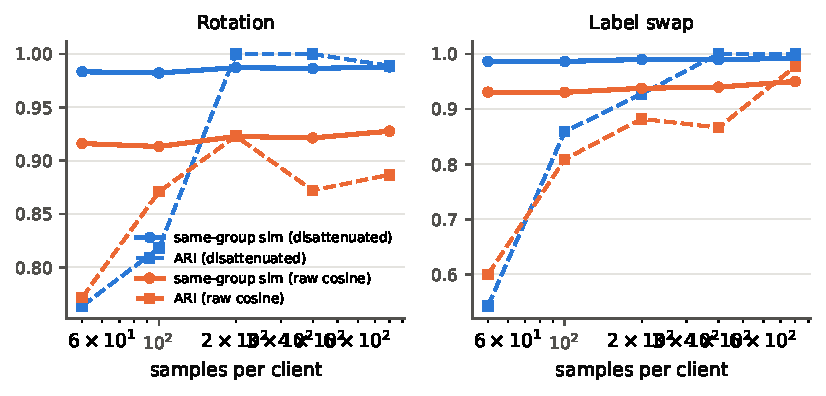
\includegraphics[width=0.85\linewidth]{../results/figures/sample_size.pdf}
\caption{Same-group similarity (solid) and ARI (dashed) as a function of the client size. Blue: disattenuated; orange: raw cosine.}\label{fig:size}
\end{figure}
\begin{figure}[!htbp]
\centering
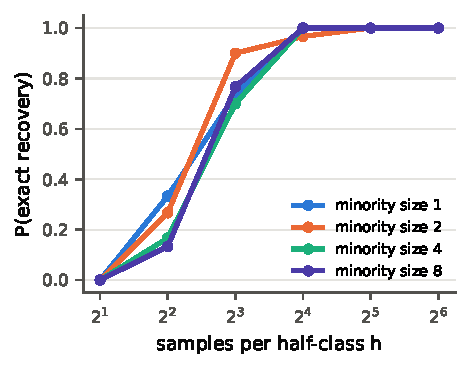
\includegraphics[width=0.45\linewidth]{../results/figures/theory_minority.pdf}
\caption{Synthetic validation of Corollary~\ref{cor:sc}: exact recovery of a minority group does not depend on its size.}\label{fig:thminority}
\end{figure}
\begin{table}[h]
\centering
\caption{Sensitivity to the shrinkage $\lambda$ at $\tau=0.8$: ARI / number of clusters (3 seeds, clustering step). For the label-only scenario the correct $K$ is 1.}\label{tab:lambda}
\small
\begin{tabular}{lccccc}
\toprule
Scenario & $\lambda=0.02$ & $\lambda=0.1$ & $\lambda=0.2$ & $\lambda=0.5$ & $\lambda=1.0$ \\
\midrule
Rotation & 1.00 / 4.0 & 1.00 / 4.0 & 1.00 / 4.0 & 1.00 / 4.0 & 0.98 / 4.0 \\
Label swap & 1.00 / 4.0 & 1.00 / 4.0 & 1.00 / 4.0 & 1.00 / 4.0 & 1.00 / 4.0 \\
Rotation + QS & 0.99 / 4.3 & 0.99 / 4.3 & 0.99 / 4.3 & 1.00 / 4.0 & 0.98 / 4.0 \\
Mixed + QS & 0.96 / 4.0 & 0.94 / 4.0 & 0.94 / 4.0 & 0.94 / 4.0 & 0.91 / 4.0 \\
Label skew only & 0.67 / 1.3 & 0.67 / 1.3 & 0.67 / 1.3 & 0.67 / 1.3 & 0.67 / 1.3 \\
Minority groups & 0.98 / 4.3 & 0.98 / 4.3 & 0.98 / 4.3 & 0.98 / 4.3 & 1.00 / 4.0 \\
\bottomrule
\end{tabular}
\end{table}


\subsection{Cost and scalability}\label{sec:cost}
Each client uploads its signature \emph{once}, about $1.2\times10^4$ floats with $p=1024$. The size is independent of the model dimension $d$; IFCA, by contrast, downloads $K$ models per client in \emph{every} round, and CFL/FL+HC cluster $d$-dimensional updates. Computing the signature takes 0.14--0.16\,s per client on one CPU core. Server-side clustering takes 0.05\,s for 40 clients and 2.3\,s for 320 clients, with ARI $\ge0.98$ at every scale.
